% !TEX TS-program = pdflatex
% !TEX encoding = UTF-8 Unicode

% This is a simple template for a LaTeX document using the "article" class.
% See "book", "report", "letter" for other types of document.

\documentclass[11pt,twoside,onecolumn,openany]{book} % use larger type; default would be 10pt
%\documentclass[12pt,twoside,onecolumn,openany]{book}

\usepackage[spanish,activeacute]{babel}
\usepackage[utf8]{inputenc} % set input encoding (not needed with XeLaTeX)

%%% Examples of Article customizations
% These packages are optional, depending whether you want the features they provide.
% See the LaTeX Companion or other references for full information.

%%% PAGE DIMENSIONS
\usepackage{geometry} % to change the page dimensions
\geometry{letterpaper} % or letterpaper (US) or a5paper or....
% \geometry{margins=2in} % for example, change the margins to 2 inches all round
% \geometry{landscape} % set up the page for landscape
%   read geometry.pdf for detailed page layout information

\usepackage{url}
\usepackage{multicol}
\usepackage{tikz}
\usetikzlibrary{arrows}
%\usetikzlibrary{arrows,shapes,snakes,automata,backgrounds,petri}

\usepackage{theorem}
\newtheorem{defi}{Definición}

\usepackage{fancyvrb}

%% Define a new 'leo' style for the package that will use a smaller font.
\makeatletter
\def\url@leostyle{%
  \@ifundefined{selectfont}{\def\UrlFont{\sf}}{\def\UrlFont{\small\ttfamily}}}
\makeatother
%% Now actually use the newly defined style.
\urlstyle{leo}

% Para que no divida las palabras
\pretolerance = 10000 
\tolerance = 20000

% Margenes del documento
\oddsidemargin 0.5in
\textwidth 5.75in
\topmargin 0in
\headheight 0in
\textheight 8.5in

%%% PACKAGES
\usepackage{listings}
\usepackage{booktabs} % for much better looking tables
\usepackage{array} % for better arrays (eg matrices) in maths
\usepackage{paralist} % very flexible & customisable lists (eg. enumerate/itemize, etc.)
\usepackage{verbatim} % adds environment for commenting out blocks of text & for better verbatim
\usepackage{subfig} % make it possible to include more than one captioned figure/table in a single float
% These packages are all incorporated in the memoir class to one degree or another...

%\usepackage{amsmath}
\usepackage[all]{xy}

%\usepackage{subfigure}
%\usepackage[refpages]{gloss}
%\usepackage{tikz}
%\usetikzlibrary{arrows,automata}
%\usepackage{amsmath}
\usepackage{pdfpages} % to import PDF pages
\usepackage{graphicx} % support the \includegraphics command and options
% \usepackage[parfill]{parskip} % Activate to begin paragraphs with an empty line rather than an indent
%\usepackage{pstricks}
%\usepackage{pst-all}
\usepackage{amssymb}
\usepackage[lined,,commentsnumbered]{algorithm2e}
%\usepackage{graphicx}% http://ctan.org/pkg/graphicx
\usepackage{subfig}% http://ctan.org/pkg/subfig

\usetikzlibrary{automata} % LATEX and plain TEX 
\usetikzlibrary[automata] % ConTEXt

%%% HEADERS & FOOTERS
\usepackage{fancyhdr} % This should be set AFTER setting up the page geometry
\pagestyle{fancy} % options: empty , plain , fancy
\renewcommand{\headrulewidth}{0pt} % customise the layout...
\lhead{}\chead{}\rhead{}
\lfoot{}\cfoot{\thepage}\rfoot{}

%%% SECTION TITLE APPEARANCE
\usepackage{sectsty}
\allsectionsfont{\sffamily\mdseries\upshape} % (See the fntguide.pdf for font help)

\setcounter{secnumdepth}{3} % para que ponga 1.1.1.1 en subsubsecciones...
\setcounter{tocdepth}{4} % para que añada las subsubsecciones y párrafos en el indice...
% (This matches ConTeXt defaults)

\usepackage[nottoc,notlof,notlot]{tocbibind} % Put the bibliography in the ToC
\usepackage[titles,subfigure]{tocloft} % Alter the style of the Table of Contents
\renewcommand{\cftsecfont}{\rmfamily\mdseries\upshape}
\renewcommand{\cftsecpagefont}{\rmfamily\mdseries\upshape} % No bold!
%%% END Article customizations

%%% The "real" document content comes below...

\title{UNIVERSIDAD AUTÓNOMA DE SAN LUIS POTOSÍ \\Facultad de Ingeniería \\Área de Computación e Informática \\ \vspace{2.0cm}
\bf ``Organizaciones de Archivos"}

\author{por\\ \\{\Large\bf {Lara Moreno Jesús Alejandro}} \\{\Large\bf {Alejandra}} \\ \\ \\ \\ \\
{\large Ing. Gerardo Padilla Lomelí} \\ {\small Profesor}\\ \\ \\ \\ REPORTE DE PROYECTO PARA LA MATERIA\\ DE ESTRUCTURAS DE ARCHIVOS}

\date{Septiembre, 2016}

\newenvironment{changemargin}[3]{% 
\begin{list}{}{% 
\setlength{\topsep}{0pt}%
\setlength{\topmargin}{#1}% 
\setlength{\leftmargin}{#2}% 
\setlength{\rightmargin}{#3}% 
\setlength{\listparindent}{\parindent}% 
\setlength{\itemindent}{\parindent}% 
\setlength{\parsep}{\parskip}% 
}% 
\item[]}{\end{list}} 

\begin{document}
\maketitle

\pagenumbering{roman} % para comenzar la numeración de paginas en números romanos
%\thispagestyle{empty} % para quitar el numero de página

\renewcommand{\listtablename}{Índice de tablas}
\renewcommand{\tablename}{Tabla}

\tableofcontents % indice de contenidos
\addcontentsline{toc}{chapter}{Estructuras de archivos} % para que aparezca en el indice de contenidos

% Secciones del documento, incluir el nombre del archivo sin extensión de la carpeta secciones
\chapter[Introducción]{Introducción}
\pagenumbering{arabic} % para empezar la numeración con números

Un aspecto fundamental de los sistemas de información es la organización sobre la cual maneja sus datos ya que de ello depende el desempeño de los programas. En el siguiente contenido desarrollaremos teórica y prácticamente las diferentes organizaciones de archivos, las cuales implementamos para diccionario de datos.


\chapter[Conceptos]{Conceptos}

\section{Archivo}
Un archivo es una colección de registros logicamente relacionados. Por lo	regular, todos los registros de un archivo	tienen un formato único, aunque existen archivos con multiples	 formatos de registros.	

\section{Entidad}
Las entidades se describen en la estructura de la base de datos empleando un modelo de datos.
Cada entidad está constituida por uno o más atributos. Por ejemplo, la entidad "Alumno" podría tener los atributos: nombre, apellido, año de nacimiento, etc.

\section{Atributos}
Los atributos son las características por medio de los cuales se puede describir una entidad.

\section{Datos}
Un dato es una representación simbólica (numérica, alfabética, algorítmica, espacial, etc.) de un atributo o variable cuantitativa o cualitativa. Los datos describen hechos empíricos, sucesos y entidades.

\chapter[Organizaciones de archivos]{Organizaciones de archivos}

Las técnicas utilizadas para representar y almacenar registros en archivos se llama organización de archivos. Las cuatro técnicas fundamentales de organización de archivos que analizaremos son las siguientes:
\begin{itemize}
\item Secuencial 
\item Secuencial indexado
\item Archivos indexados con arboles b+
\item Archivos directos con (hash dinámica)
\item Archivos directos con (hash estática)
\item Organización de archivos multillave
\end{itemize}

\chapter[Operaciones sobre archivo]{Operaciones sobre archivo}

La manera como se usar el archivo es un factor importante para determinar como se debe organizar el archivo. Dos aspectos importantes sobre el uso de archivos son su modo de utilización y la naturaleza de las operaciones sobre el archivo.
Las operaciones básicas que se ejecutan sobre los archivos son las siguientes:

\begin{itemize}
\item[1.] Creación
\item[2.] Actualización, incluyendo:
\begin{itemize}
\item[a.] inserción de registros
\item[b.] modificación de registros
\item[c.] supresión de registros
\end{itemize}
\item[3.] Recuperación incluyendo:
\begin{itemize}
\item[a.] Consulta
\item[b.] Generación de reportes
\end{itemize}
\item[4.] Mantenimiento, incluyendo:
\begin{itemize}
\item[a. ] Estructuración 
\item[b. ] Reorganización
\end{itemize}
\end{itemize}

\section{Creación de un archivo}

La creación inicial de un archivo es conocida también como la carga del archivo.
El grueso del trabajo en la creación de archivos incluye la validación de datos. En algunas implantaciones, primero se asigna el espacio para el archivo y después los datos son cargados dentro de ese “esqueleto” de archivo. En otras implantaciones, el archivo se construye registro por registro.

\newpage
\lstset{language=C++, breaklines=true, basicstyle=\footnotesize, basewidth  = {.5em,0.4em}}
\begin{lstlisting}[frame=single]
string CDiccionario::abrir_Diccionario(char n[20]) {
    std::stringstream buffer;
    CEntidad aux_entidad;
    long auxDir_siguiente;
    this->lista_entidades.clear();
    //Si el archivo esta abierto se cierra
    if(this->ptr_Archivo != NULL) {
        std::fclose(this->ptr_Archivo);
        this->cabecera = -1;
    }
    /*Se abre el archivo considerando que existe*/
    this->ptr_Archivo = std::fopen(n, "r+b");
    /*Si el archivo se pudo abrir se cargan sus datos*/
    if(this->ptr_Archivo != NULL) {
        buffer << "Diccionario " << n << " Abierto!!";
        /*Se lee su cabecera en el archivo y sea actualiza la cabecera de la clase*/
        std::fread(&this->cabecera, sizeof(long), 1, this->ptr_Archivo);
        buffer << " Cabecera en " << this->cabecera  << std::endl;
        /*Se cargas todos sus Entidades y atributos*/
        if(this->cabecera != -1) {
            std::fseek(this->ptr_Archivo, this->cabecera, SEEK_SET);
            std::fread(&aux_entidad, sizeof(CEntidad), 1, this->ptr_Archivo);
            aux_entidad.inicia_ListaAtributos();
            aux_entidad.carga_Atributos(this->ptr_Archivo);
            this->lista_entidades.push_back(aux_entidad);
            while(aux_entidad.dameDir_Siguiente() != -1) {
                auxDir_siguiente = aux_entidad.dameDir_Siguiente();
                std::fseek(this->ptr_Archivo, auxDir_siguiente, SEEK_SET);
                std::fread(&aux_entidad, sizeof(CEntidad), 1, this->ptr_Archivo);
                aux_entidad.inicia_ListaAtributos();
                aux_entidad.carga_Atributos(this->ptr_Archivo);
                this->lista_entidades.push_back(aux_entidad);
            }
            /*Cargadas todas las entidades se ordena la lista*/
            this->lista_entidades.sort();
        }
    }
    /*Si el archivo no se pudo abrir se crea automaticamente*/
    else {
        this->ptr_Archivo = std::fopen(n, "w+b");
        /*Si el archivo se pudo crear*/
        if(this->ptr_Archivo != NULL) {
        	buffer << "Diccionario " << n << " Creado!!" << std::endl;
            /*Escribimos la cabecera vacia en el archivo nuevo*/
            std::fwrite(&this->cabecera, sizeof(long), 1, this->ptr_Archivo);
        }
        /*Si no se pudo crear el diccionario*/
        else {
            buffer << "No se pudo crear el diccionario " << n << std::endl;
        }
    }return buffer.str();
}
\end{lstlisting}

\section{Actualización de un archivo}

Cambiar el contenido de un archivo maestro para hacer que refleje un momento transitorio mas actual del mundo real es a lo cual se llama, actualización de archivos.
\begin{itemize}
\item[1.] La inserción de nuevos registros, por ejemplo, la edición de un registro para un empleado de nuevo ingreso a la compañía.
\item[2.] La modificación de datos a registros que ya existen en el archivo, por ejemplo, cambiar el sueldo del empleado, cambiar el indicativo de estado del empleado(activo, no activo, de licencia)
\item[3.] La supresión de registros del archivo, esto es, borrar el registro de un empleado que salió de la compañía. 
\end{itemize}

De esta manera el archivo muestra una imagen mas actual de la realidad.

\section{Recuperación de información de un archivo}

El acceso a un archivo con el propósito de extraer información significativa es llamado recuperación de información. Existen dos clases de recuperación de información: consultas y generación de reportes. Estas dos clases pueden distinguir de acuerdo a volumen de información que producen. Una consulta produce un volumen relativamente mínimo, mientras que un reporte puede crear muchas paginas de salida de información.

\section{Mantenimientos de archivos}

Cambios hechos sobre archivos para mejorar la eficiencia de los programas que los accesan son los conocidos como actividades de mantenimiento. Existen dos clases de operaciones de mantenimiento básicas, las cuales son: reestructuración y reorganización. La reestructuración de un archivo implica que es necesario aplicar cambios estructurales, dentro del contexto de la misma técnica de organización de archivos. La reorganización implica cambiar la organización de un archivo a otro tipo de organización.

\chapter[Diccionario de datos]{Diccionario de datos}
Es un conjunto de metadatos que contiene las características lógicas y puntuales de los datos que se van a utilizar en un sistema que se programa, incluyendo nombres, descripción, alias, contenido y organización.

\section{Descripción de un diccionario de datos}
Es un catálogo de los elementos en un sistema. Como su nombre lo sugiere, estos elementos se centran alrededor de los datos y la forma en que están estructurados para satisfacer los requerimientos de los usuarios y las necesidades de la organización. En un diccionario de datos se encuentra la lista de todos los elementos que forman parte del flujo de datos en todo el sistema. Los elementos más importantes son flujos de datos, almacenes de datos y procesos. El diccionario guarda los detalles y descripciones de todos estos elementos.

\section{Operaciones basicas de un diccionario de datos}
\begin{itemize}

\item[•] Altas
\begin{itemize}
\item[-] La modificación de datos a registros que ya existen en el archivo, por ejemplo, cambiar el sueldo del empleado, cambiar el indicativo de estado del empleado(activo, no activo, de licencia)
\end{itemize}
\item[•] Bajas
\begin{itemize}
\item[-] La supresión de registros del archivo, esto es, borrar el registro de un empleado que salió de la compañía.
\end{itemize}
\item[•] Modificaciones
\begin{itemize}
\item[-] La modificación de datos a registros que ya existen en el archivo, por ejemplo, cambiar el sueldo del empleado, cambiar el indicativo de estado del empleado(activo, no activo, de licencia)
\end{itemize}
\end{itemize}

\section{Ejemplos}

\subsection{Altas}
\begin{figure}[!ht]
\begin{center}
  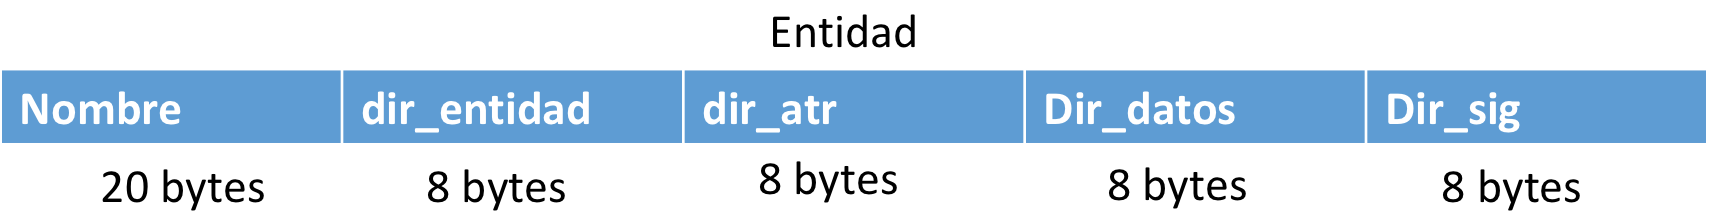
\includegraphics[width=0.5\textwidth]{secciones/ejemploA/img1.png}
  \caption{Campos de una entidad}
\end{center}
\end{figure}
\begin{figure}[!ht]
\begin{center}
  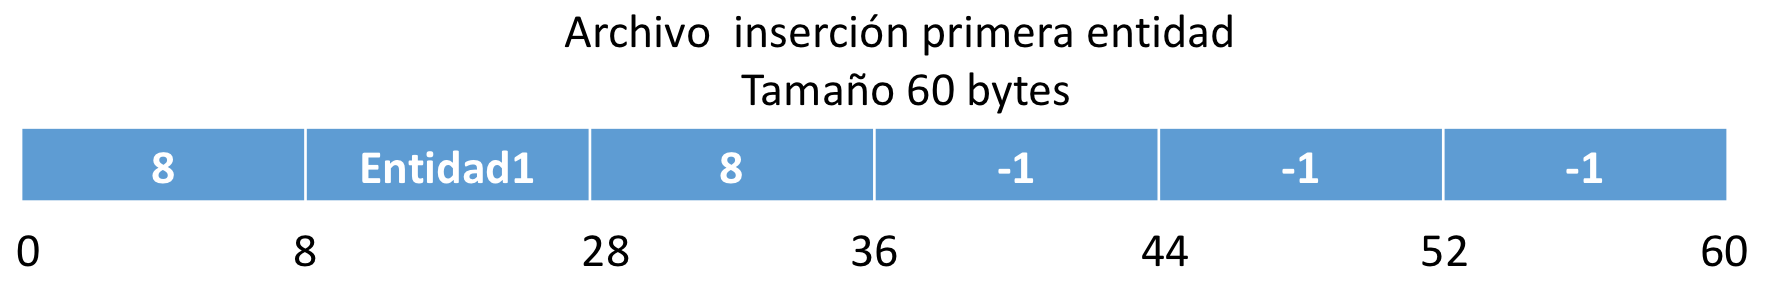
\includegraphics[width=0.5\textwidth]{secciones/ejemploA/img2.png}
  \caption{Insercion primera de una entidad en el diccionario.}
\end{center}
\end{figure}
\begin{figure}[!ht]
\begin{center}
  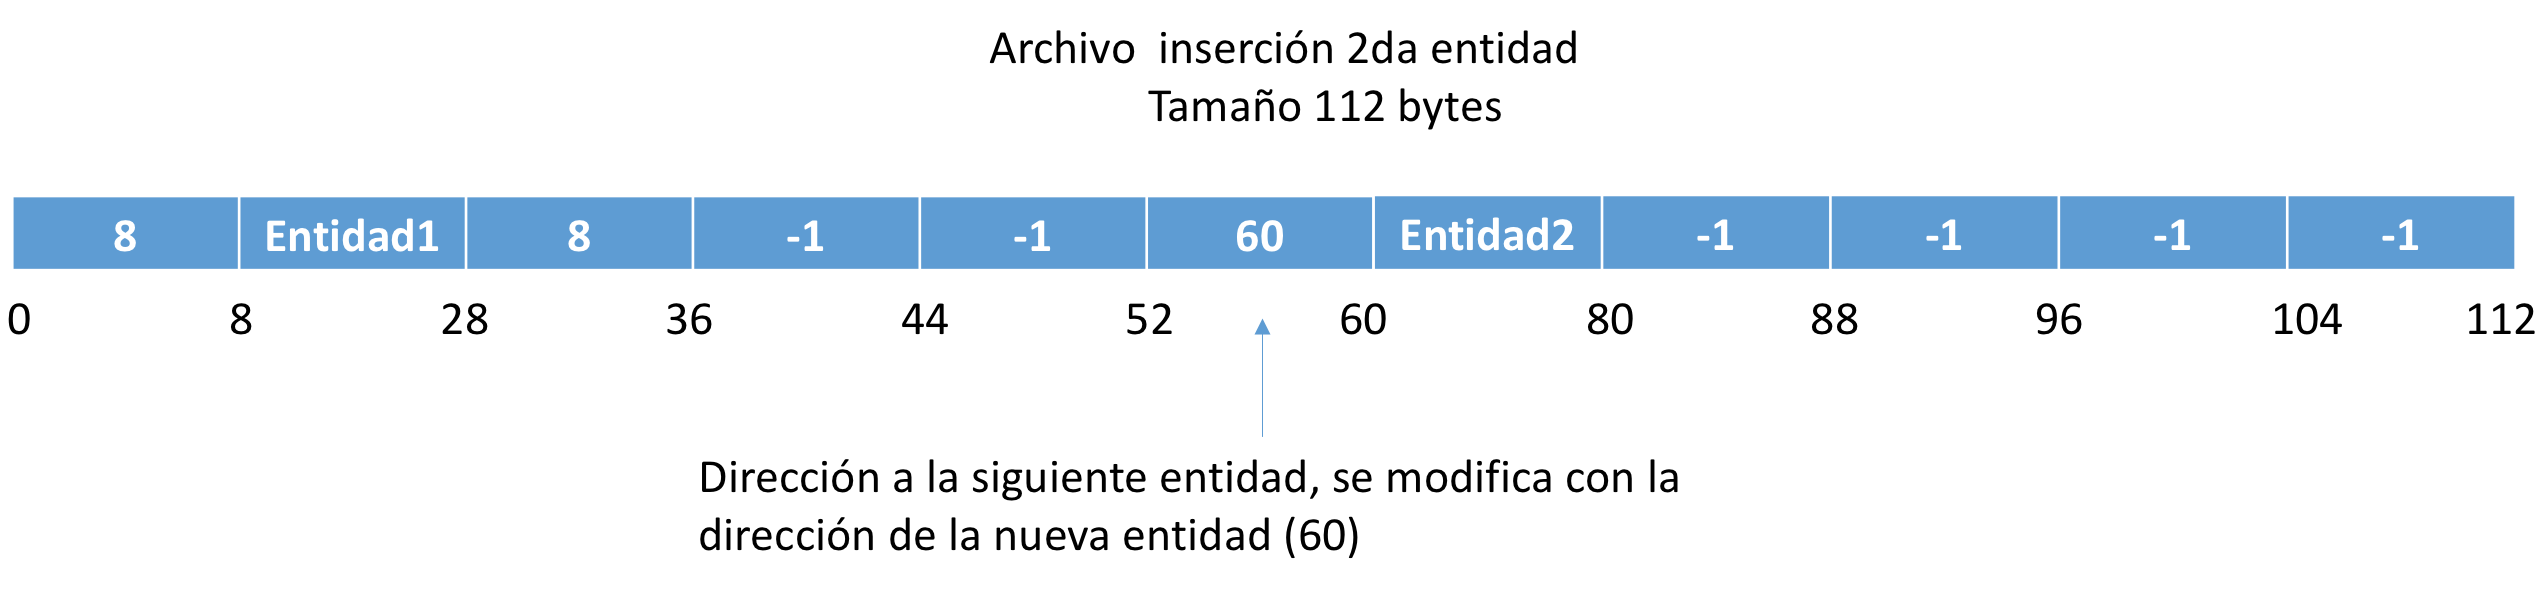
\includegraphics[width=0.5\textwidth]{secciones/ejemploA/img3.png}
  \caption{Insercion segunda de una entidad en el diccionario.}
\end{center}
\end{figure}
\begin{figure}[!ht]
\begin{center}
  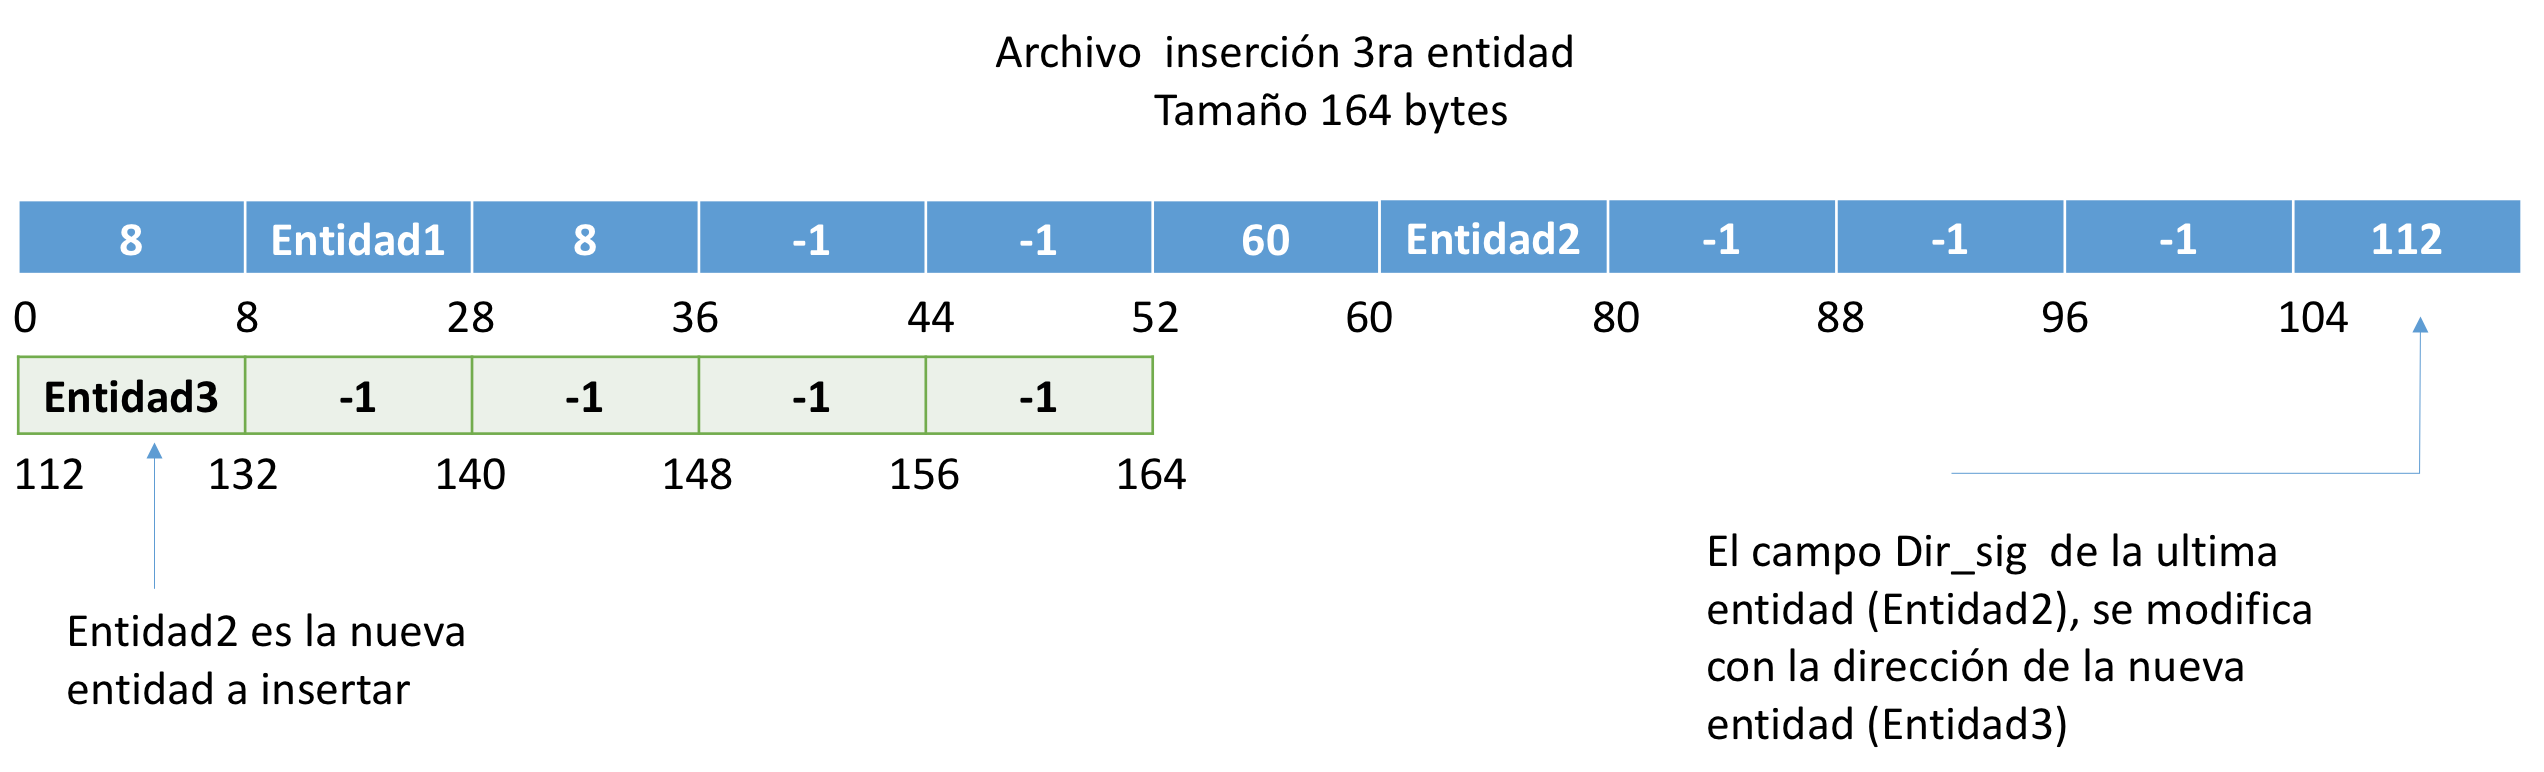
\includegraphics[width=0.5\textwidth]{secciones/ejemploA/img4.png}
  \caption{Insercion tercera de una entidad en el diccionario.}
\end{center}
\end{figure}

\newpage
\subsection{Codigo en C++ de Altas}
\lstset{language=C++, breaklines=true, basicstyle=\footnotesize, basewidth  = {.5em,0.4em}}
\begin{lstlisting}[frame=single]
string CDiccionario::agrega_Entidad(char n[20])
{
    long dir_nueva;
    std::stringstream buffer;
    CEntidad *nueva_entidad, aux_entidad;
    std::list<CEntidad>::iterator atras_entidad;

    if(this->ptr_Archivo != NULL)
    {
        /*Se pone el apuntador al final de archivo*/
        std::fseek(this->ptr_Archivo, 0, SEEK_END);
        dir_nueva = std::ftell(this->ptr_Archivo);
        nueva_entidad = new CEntidad(n, dir_nueva);
        std::fwrite(nueva_entidad, sizeof(CEntidad), 1, this->ptr_Archivo);

        //Si el diccionario esta vacio agrega y actualiza la cabecera
        if(this->lista_entidades.empty())
        {
            this->cabecera = dir_nueva;
            //Se actualiza la cabecera en el archivo
            std::fseek(this->ptr_Archivo, 0, SEEK_SET);
            std::fwrite(&this->cabecera, sizeof(long), 1, this->ptr_Archivo);
            //Se agrega la nueva entidad a la lista
            this->lista_entidades.push_back(*nueva_entidad);
            buffer << "Se agrego la entidad " << n << " al diccionario" << std::endl;

        }
        else
        {
            //recorre la lista y busca el ultimo elemento
            atras_entidad = this->lista_entidades.begin();
            while(atras_entidad != this->lista_entidades.end()
                  && atras_entidad->dameDir_Siguiente() != -1)
            {
                atras_entidad++;
            }
            //Verifica si encontro la ultima entidad al final
            if(atras_entidad->dameDir_Siguiente() == -1)
            {
                std::fseek(this->ptr_Archivo, atras_entidad->dameDir_Entidad(), SEEK_SET);
                atras_entidad->ponDir_Siguiente(dir_nueva);
                aux_entidad = *atras_entidad;
                std::fwrite(&aux_entidad, sizeof(CEntidad), 1, this->ptr_Archivo);
                this->lista_entidades.push_back(*nueva_entidad);
                buffer << "Se agrego la entidad " << n << " al diccionario" << std::endl;
            }
        }
        //Ordena a lista por nombres, esto es posible por la sobrecarga del operador ==
        this->lista_entidades.sort();
    }
    //Retorna un buffer que despues es mostrado al inicio del menu.
    return buffer.str();
\end{lstlisting}

\subsection{Bajas}
\begin{figure}[!ht]
\begin{center}
  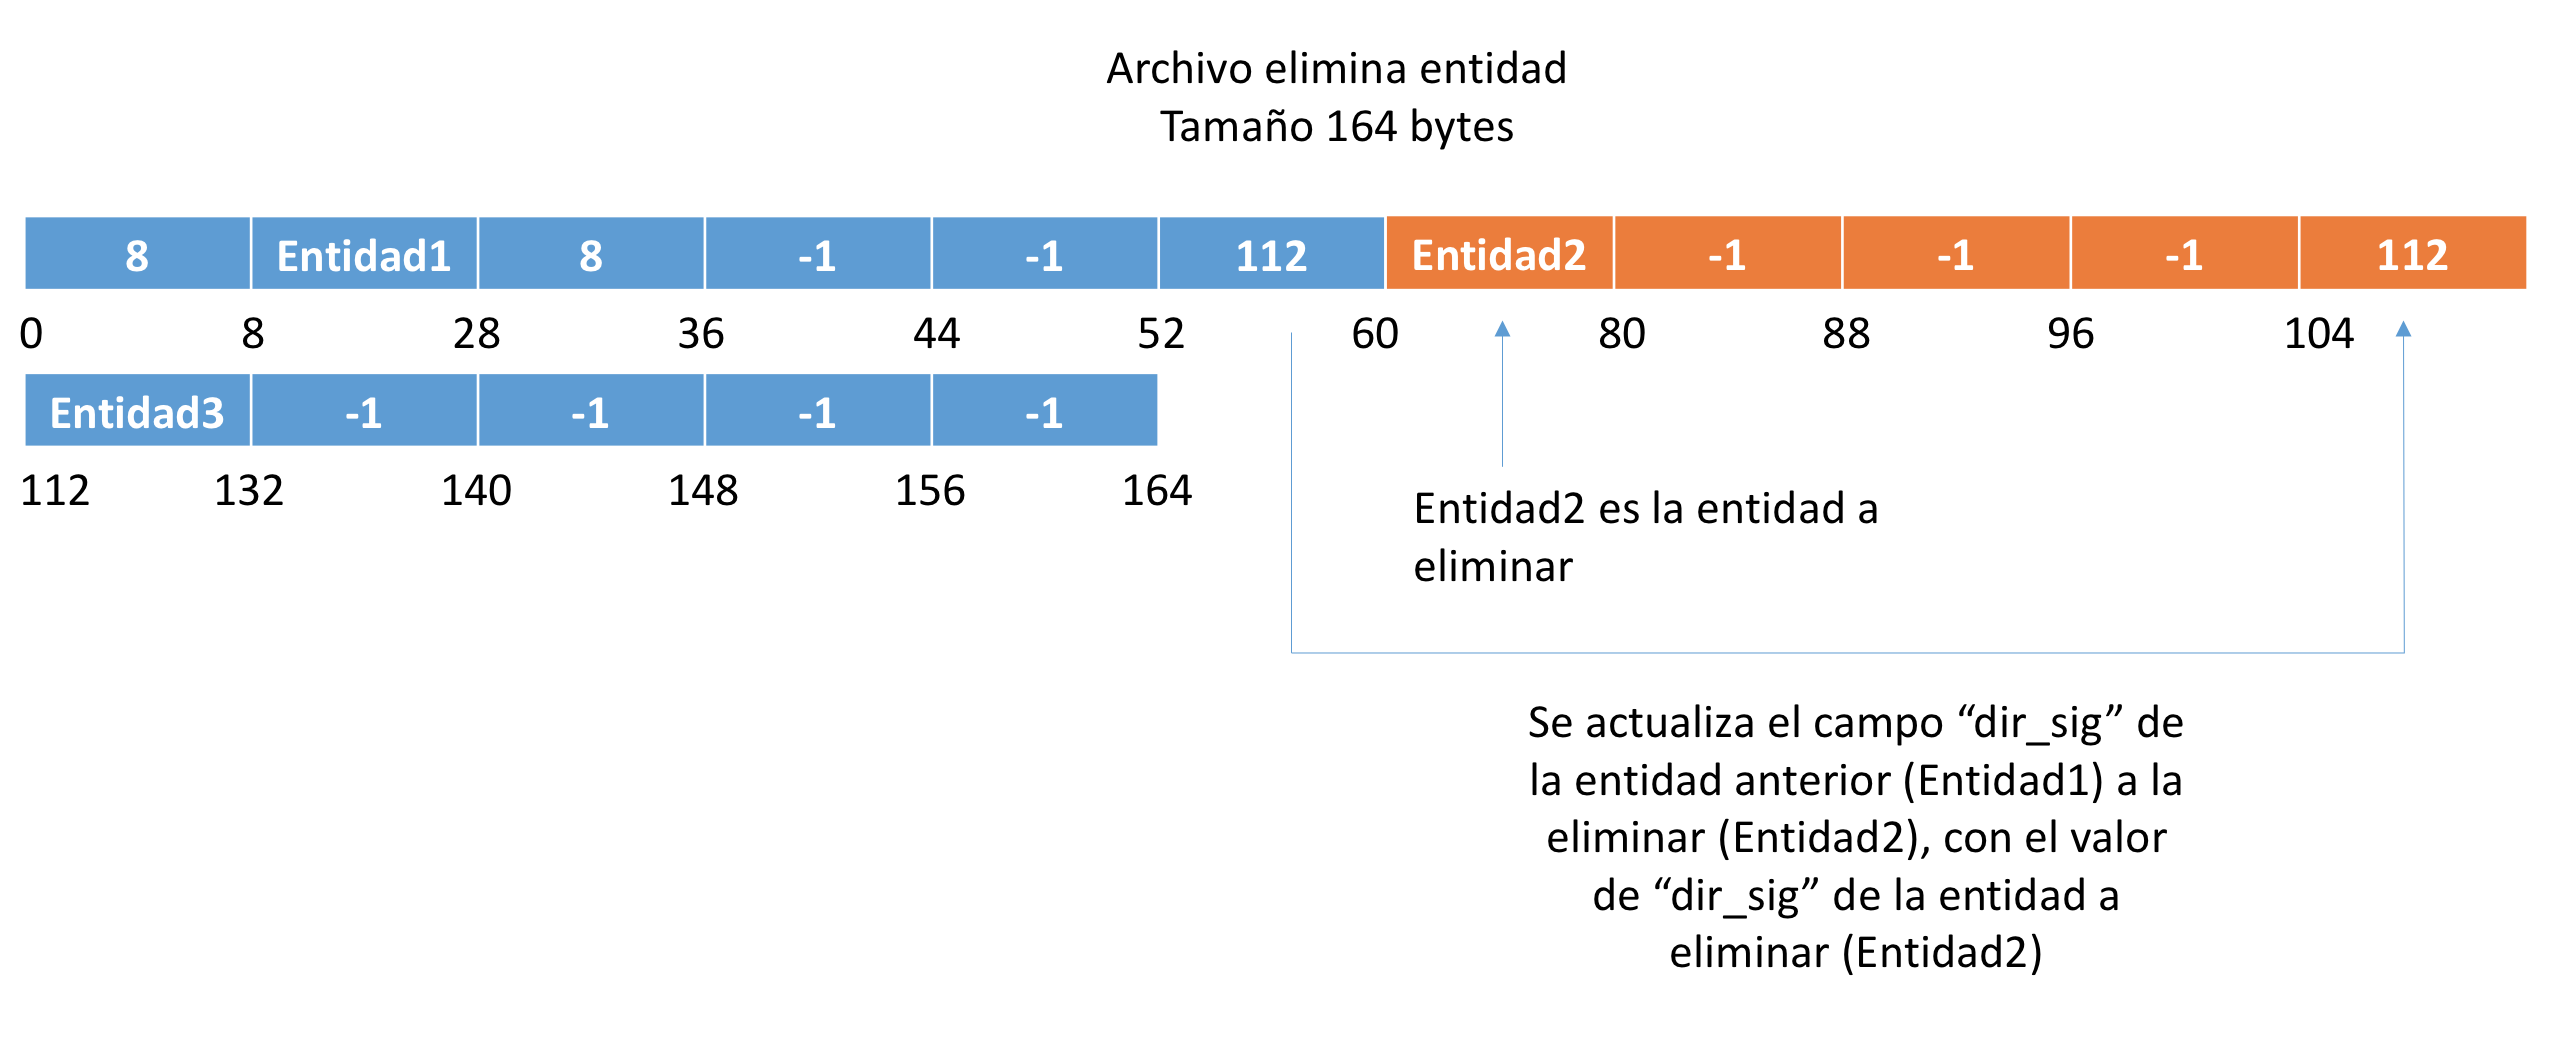
\includegraphics[width=0.5\textwidth]{secciones/ejemploA/Elimina1.png}
  \caption{Eliminación de un campo, la eliminación solo se actualizan los apuntadores.}
\end{center}
\end{figure}
\begin{figure}[!ht]
\begin{center}
  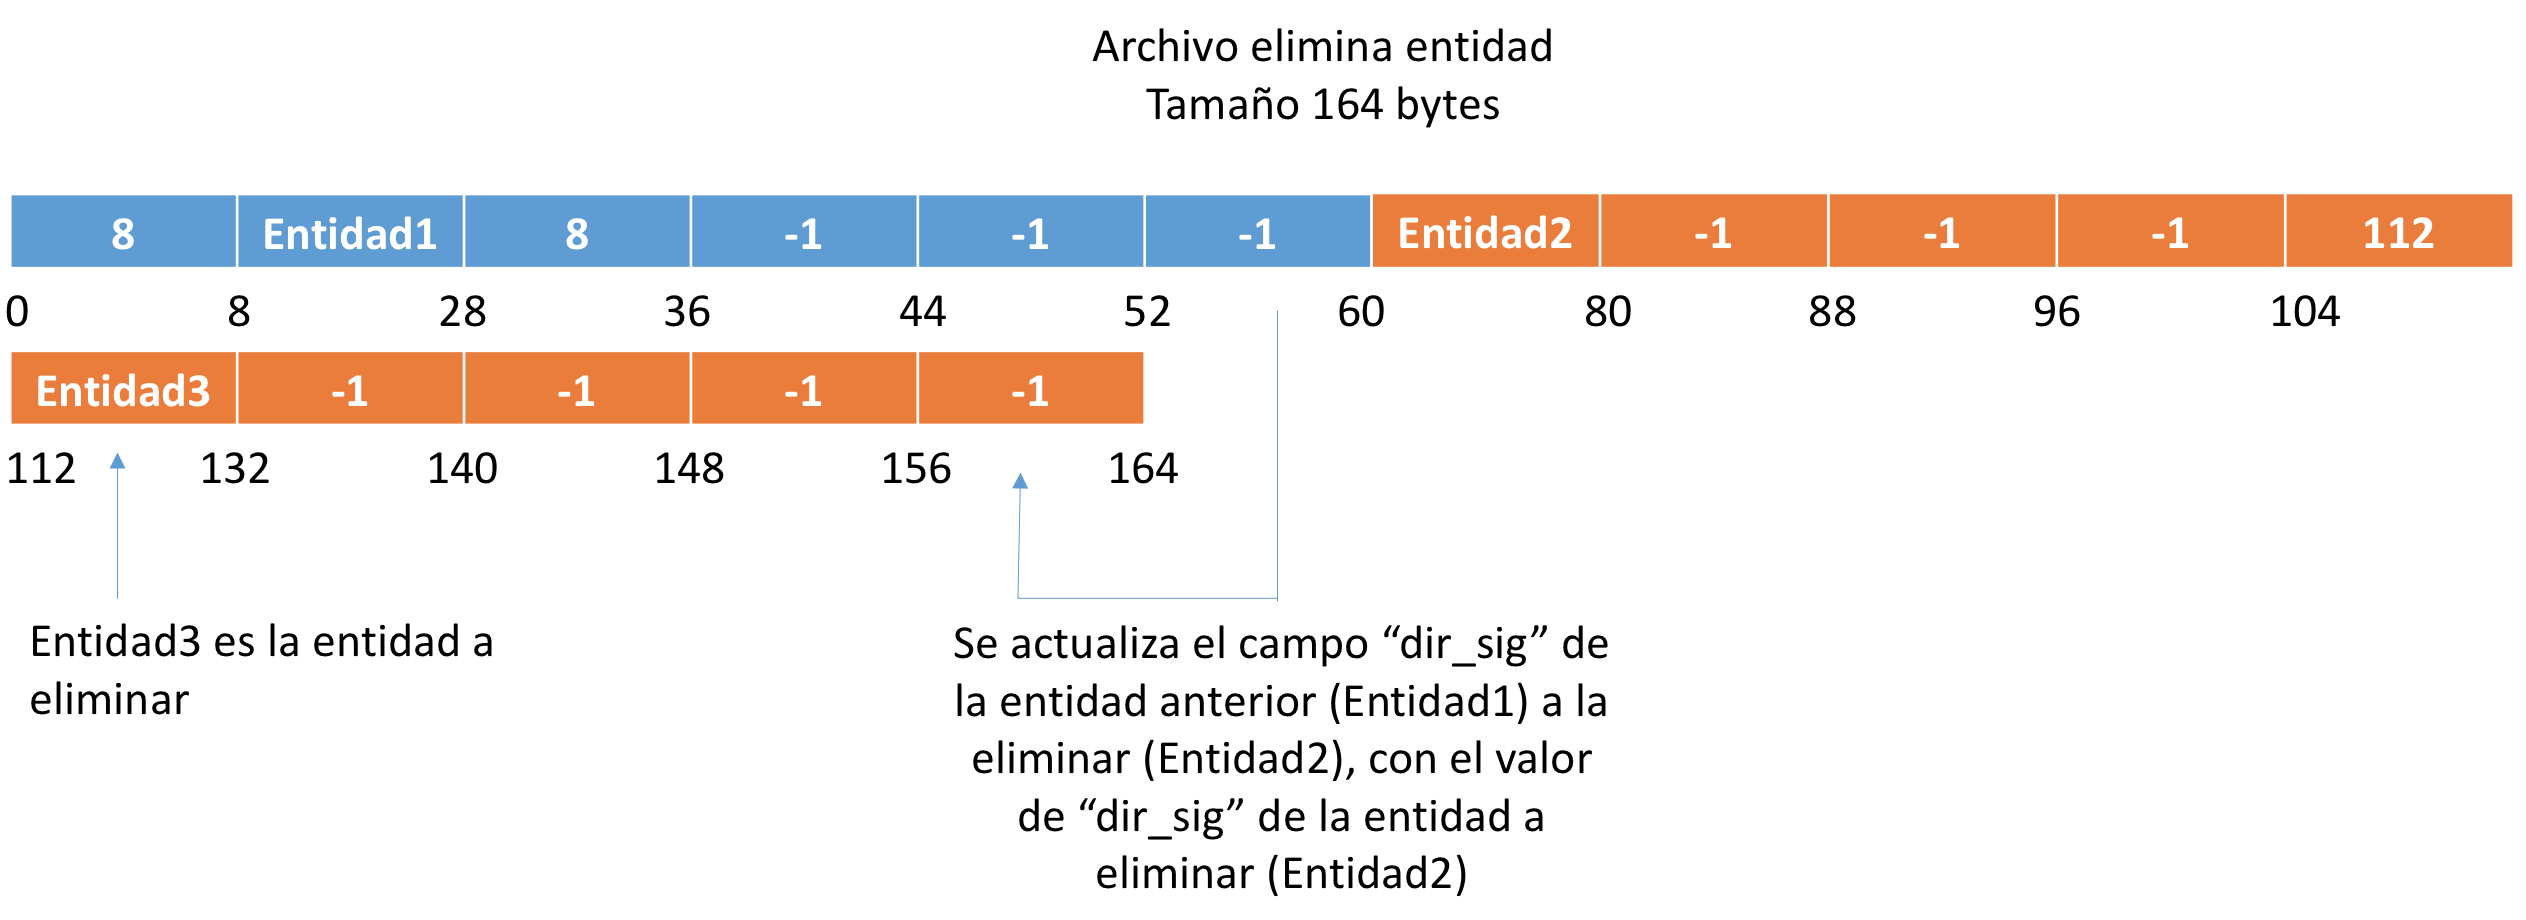
\includegraphics[width=0.5\textwidth]{secciones/ejemploA/Elimina2.png}
  \caption{Eliminación al final del diccionario.}
\end{center}
\end{figure}
\begin{figure}[!ht]
\begin{center}
  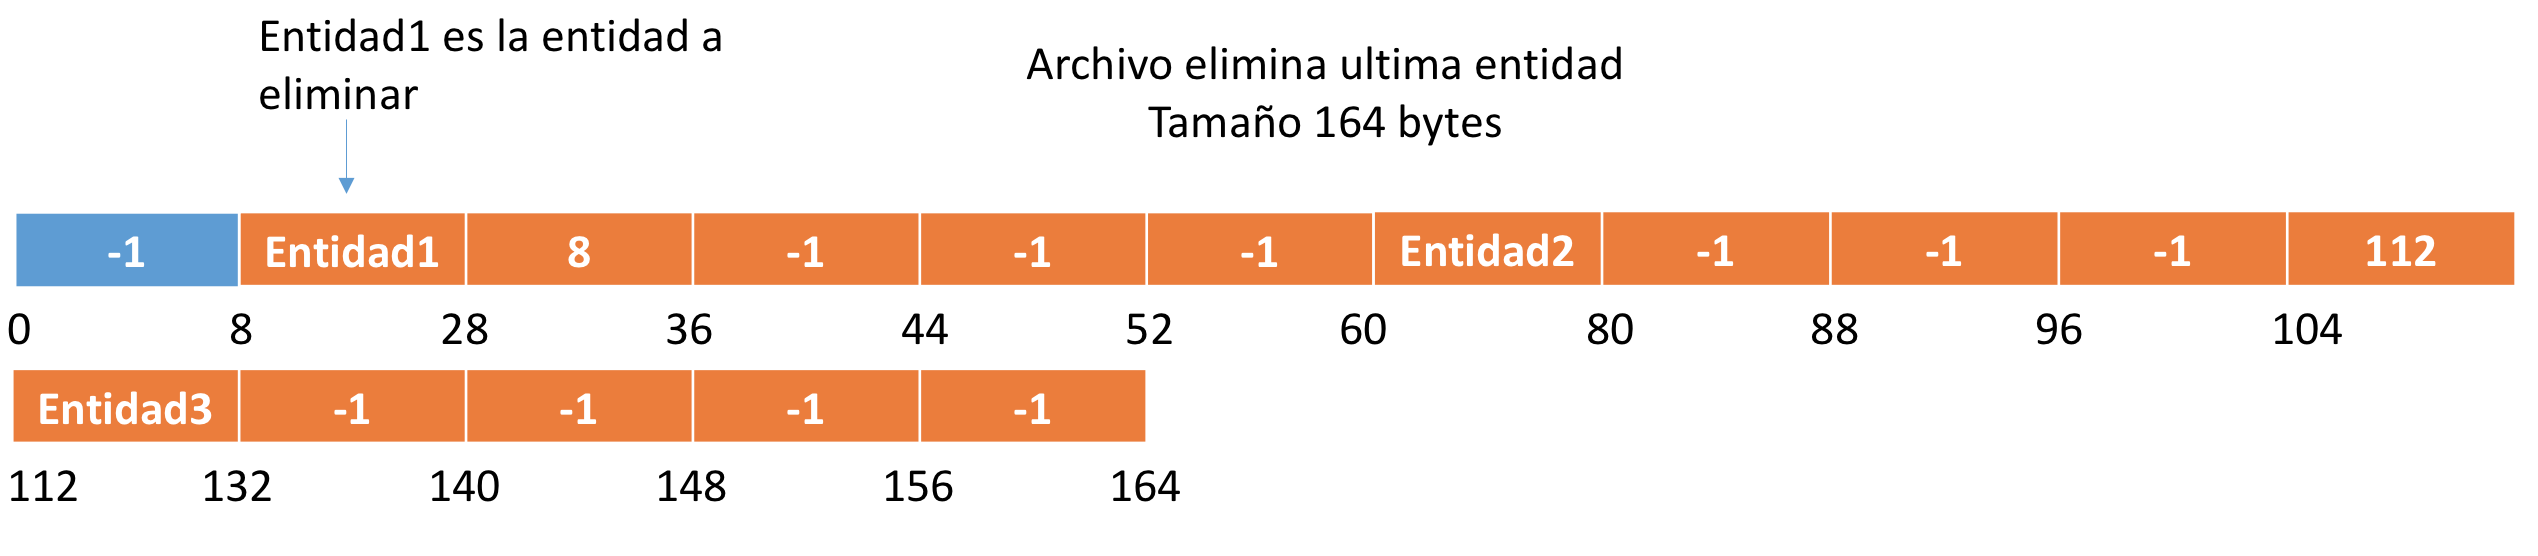
\includegraphics[width=0.5\textwidth]{secciones/ejemploA/Elimina3.png}
  \caption{Eliminación al inicio del diccionario.}
\end{center}
\end{figure}

\newpage
\subsection{Codigo en C++ de Bajas}
\lstset{language=C++, breaklines=true, basicstyle=\footnotesize, basewidth  = {.5em,0.4em}}
\begin{lstlisting}[frame=single]
string CDiccionario::elimina_Entidad(int n) {
    std::stringstream buffer;
    CEntidad aux_entidad;
    std::list<CEntidad>::iterator iterador;
	/*Si el archivo esta creado entra para realizarla baja*/
    if(this->ptr_Archivo != NULL) {
    	/*Se ubica el iterador en la primera entidad de la lista*/
        iterador = this->lista_entidades.begin();
        if(iterador != this->lista_entidades.end()) {
        	/*Avanza el iterador segun el index*/
            std::advance(iterador, n);
            aux_entidad = *iterador;

            iterador = this->lista_entidades.begin();
            while((iterador->dameDir_Siguiente() != aux_entidad.dameDir_Entidad())
                  && iterador != this->lista_entidades.end()) {
                iterador++;
            }
            /*Si el iterador es correcto modifica el archivo*/
            if(iterador->dameDir_Siguiente() == aux_entidad.dameDir_Entidad())
            {
                buffer << "Encontro el anterior " << iterador->dame_Nombre() << std::endl;
                iterador->ponDir_Siguiente(aux_entidad.dameDir_Siguiente());
                std::fseek(this->ptr_Archivo, iterador->dameDir_Entidad(), SEEK_SET);
                aux_entidad = *iterador;
                std::fwrite(&aux_entidad, sizeof(CEntidad), 1, this->ptr_Archivo);
                /*Elimino la entidad de la lista*/
                iterador = this->lista_entidades.begin();
                std::advance(iterador, n);
                this->lista_entidades.remove(*iterador);
            }
            else if(this->cabecera == aux_entidad.dameDir_Entidad()) {
                this->cabecera = aux_entidad.dameDir_Siguiente();
                std::fseek(this->ptr_Archivo, 0, SEEK_SET);
                std::fwrite(&this->cabecera, sizeof(long), 1, this->ptr_Archivo);
                buffer << "Es es el primero" << iterador->dame_Nombre() << std::endl;
                /*Elimino la entidad de la lista*/
                iterador = this->lista_entidades.begin();
                std::advance(iterador, n);
                this->lista_entidades.remove(*iterador);
            }
        }
        else {
            std::cout << "El diccionario esta vacio" << std::endl;
        }
    }
    return buffer.str();
}
\end{lstlisting}

\subsection{Modificaciones}
\newpage
\subsection{Codigo en C++ de Modificaciones}
\lstset{language=C++, breaklines=true, basicstyle=\footnotesize, basewidth  = {.5em,0.4em}}
\begin{lstlisting}[frame=single]
string CDiccionario::edita_Entidad(int index, char n[20])
{
    std::stringstream buffer;
    CEntidad aux_entidad;
    char aux_nombre[20];
    std::list<CEntidad>::iterator iterador;

    if(this->ptr_Archivo != NULL)
    {
        iterador = this->lista_entidades.begin();
        /*Se verifica si la lista no esta vacia comparado el interador con el final de la
        lista*/
        if(iterador != this->lista_entidades.end())
        {
            /*El metodo advance el iterador n veces si seleccione el elemento 2
             * advance recorre el iterador 2 veces
             */
            std::advance(iterador, index-1);
            std::strcpy(aux_nombre, iterador->dame_Nombre());
            iterador->pon_Nombre(n);
            aux_entidad = *iterador;
            std::fseek(this->ptr_Archivo, iterador->dameDir_Entidad(), SEEK_SET);
            std::fwrite(&aux_entidad, sizeof(CEntidad), 1, this->ptr_Archivo);
            buffer << "Se modifico la Entidad "
                   << aux_nombre << " > " << aux_entidad.dame_Nombre()
                   << std::endl;
            this->lista_entidades.sort();
        }
        else
        {
            std::cout << "El diccionario esta vacio" << std::endl;
        }
    }
    return buffer.str();
}
\end{lstlisting}


\chapter[Organización de archivos secuenciales]{Organización de archivos secuenciales}
La manera básica de organizar un conjunto de registros, que forman un archivo, es utilizando una organización secuencial. En un archivo organizado secuencialmente, los  registros quedan grabados consecutivamente cuando el archivo se crea y deben accesarse consecutivamente cuando el archivo se usa como se muestra a continuación:

\begin{figure}[!ht]
\begin{center}
  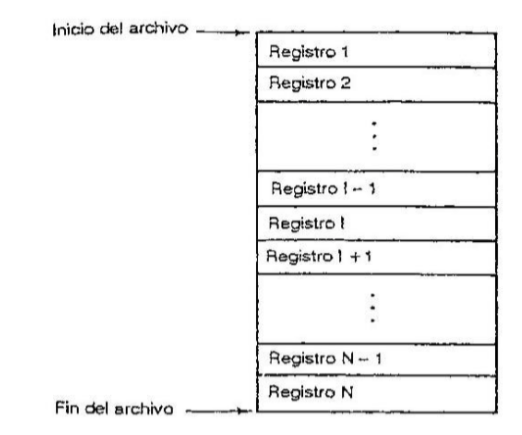
\includegraphics[width=0.5\textwidth]{secciones/imgA.png}
  \caption{Estructura de un archivo secuencial}
\end{center}
\end{figure}

En la mayoría de los casos, los registros de un archivo secuencial quedan ordenados de acuerdo con el valor de algún campo de cada registro. Semejante archivo se dice que es un archivo ordenado; el campo, o los campos, cuyo valores se utiliza para determinar el ordenamiento es conocido como llave de ordenamiento. Un archivo puede ordenarse ascendente o descendentemente con base en la llave de ordenamiento, la cual puede constar de uno o mas campos.


\begin{table}
\begin{center}

\begin{tabular}{|c|c|c|c|c|c|}
\hline
Nombre & Dir\_Entidad & Dir\_Atriuto & Dir\_Dato & Dir\_siguiente \\ 
\hline 
\end{tabular} 

\caption{Tabla de ejemplo}

\end{center}
\end{table}





%\chapter*{Apéndice A}\label{aped.A}
\markboth{APÉNDICES}{} % para que cambie el encabezado, si no, usaría el del último chapter{}
\addcontentsline{toc}{chapter}{Apendice A - Cartas de autorización de uso de información} % para que se añada en el indice

Cartas de autorización para el uso de información e imágenes de los Sistemas de Inscripciones del ITSLP {\bf (firma en tramite)} y el ITESM en esta tesis.

\begin{figure}[h]
	\centering
	\includegraphics[width=1.2\textwidth]{Carta_ITESM.pdf}
\end{figure}


%\begin{figure}[h]
%	\centering
%	\includegraphics[width=1.2\textwidth]{Carta_ITSLP.pdf}
%\end{figure}


\chapter*{Apéndice B}\label{aped.B}
\markboth{APÉNDICES}{} % para que cambie el encabezado, si no, usaría el del último chapter{}
\addcontentsline{toc}{chapter}{Apendice B - Diagrama del Modelo Entidad-Relación Mejorado} % para que se añada en el indice

Diagrama del Modelo de Entidad-Relación Mejorado de la base de datos relacional del Sistema en Línea de Inscripciones.


\begin{figure}[h]
	\centering
	\includegraphics[height=1\textheight]{D_EER_iMat.pdf}
\end{figure}



\chapter*{Apéndice C}\label{aped.C}
\markboth{APÉNDICES}{} % para que cambie el encabezado, si no, usaría el del último chapter{}
\addcontentsline{toc}{chapter}{Apendice C - Diccionario de datos} % para que se añada en el indice

Diccionario de la base de datos del Sistema en Línea de Inscripciones.

\begin{figure}[h]
	\centering
	\includegraphics[width=1.2\textwidth]{DDp1.pdf}
\end{figure}

\begin{figure}[h]
	\centering
	\includegraphics[width=1.2\textwidth]{DDp2.pdf}
\end{figure}

\begin{figure}[h]
	\centering
	\includegraphics[width=1.2\textwidth]{DDp3.pdf}
\end{figure}

\begin{figure}[h]
	\centering
	\includegraphics[width=1.2\textwidth]{DDp4.pdf}
\end{figure}

%\begin{figure}[h]
 % \centering
%\includepdf[pages={1-4}]{Diccionario.pdf}
%\end{figure}
\begin{thebibliography}{9}

%1
\bibitem{web0}
Universidad Autónoma de San Luis Potosí, {\it Antecedentes Históricos} \\
{\url{http://www.uaslp.mx/Spanish/Institucional/anthist/Paginas/default.aspx}}

%2
\bibitem{web1}
Leon Shklar, Rich Rosen, {\it Web Application Architecture: Principles, Protocols and Practices}, Auflage, 2009. [pp. 29-45]


\end{thebibliography}


\end{document}




